\chapter{Background and motivation}
\section{Cross-country skiing}
Cross-country skiing is a whole-body endurance sport where the skier uses a combination of poles and skis to generate speed across snowy terrain. This sport is used by many as a family and recreational activity, but also for more serious purpose in competitions. The goal in competitive skiing is to reach the finish line in the shortest amount of time. In modern competitions, the winning margins are very small. During a World Cup race in March 2018, the time difference between a first and fourth place varied from 1.1\% for men to 2.3\% for women on the overall standings \citep{fis_2018}. In other words, the difference between a losing and winning pair of skis in competitive skiing is minimal. The need for precise and reliable selection of professional skis increase, since selecting the best pair of skis is crucial. The importance of ski properties on performance was confirmed by Rønbeck and Vikander (2007).

\begin{figure}
    \centering
    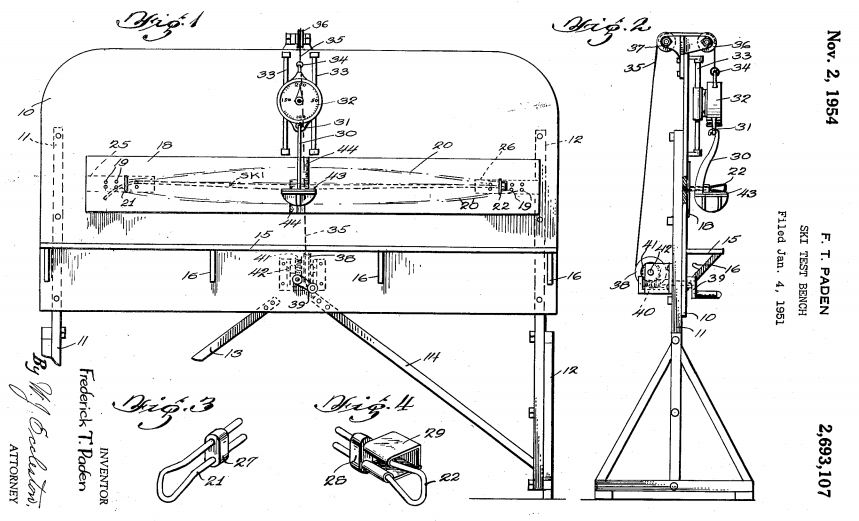
\includegraphics[width=1\textwidth]{figures/earlytb.png}
    \caption{Illustrating the concept of a test bench. Figure from \url{https://patents.google.com/patent/US2693107A/}}
    \label{fig:earlytb}
\end{figure}

The performance of a cross-country skier is highly dependent on the performance and quality of the skis. The ski's performance is determined by a number of mechanical properties such as the camber height and stiffness. These characteristics will be explained in detail later in this thesis. Another important factor for the skis performance is the wax applied under the skis, both the grip wax to make the ski grip and the gliding wax to make the ski glide. However, it is often claimed that the performance of the skis themselves are roughly 80 \% of the total performance, while the grinding of the ski sole is roughly 10 \% and the waxing also only 10 \%. 

Finding the best skis is a challenge. Skis are chosen by the athletes and the experts together to find the best fit for the athlete. Large resources and time are being spent on manually selecting a large pool of skis for testing in the field. To the author's knowledge, the skis are hand-picked straight from the manufacturers by experts with intuition and experience. These skis are stored in a pool of skis for further testing. This can indicate that the differences in each ski selected are prone to human error in terms of subjectivity. Furthermore, a quantitative way of choosing skis with mechanical measurements of the ski, can further improve the ski selection phase.

Early methods of testing mechanical properties in materials was done by applying force to the middle of a structure as shown in Figure \ref{fig:earlytb}. Testing mechanical properties in cross-country skis. In the mid-twentieth century, patents on measurement devices for measuring cross-country skis was developed. A measurement device, shown in Figure \ref{fig:earlytb} was typically used to investigate the elasticity of structures like aircraft wings or skis. The concept of this was to apply a force on the center of the structure to determine deflection or stress by the application of external forces.
Development of measurement devices have been done by companies like \textit{Skiselector} \ref{subsec:skiselector} and \textit{Gear West Signature Flex Tester} \ref{subsec:gwsft} with similar concepts. These companies uses measurement devices with the focus on measuring the height of the arch or camber and stiffness when applying external force on the balance point of the ski. After the measurement, the devices give each ski a profile with span curves, which are explained later in detail.

\subsection{Body Weights and Loading Weights}
\label{subsec:bw}
Measuring the forces applied to the ski like in the \textit{Skiselector} \ref{subsec:skiselector}, it is necessary to load the ski with the correct force for the matching ski-phase. These forces are based out of the weight of the user or skier. The necessity of using the right weight or force when measuring, is to find at which area on the ski that is allocated as the grip zone. This is done by loading the full body weight (FBW) of the skier on the ski to be measured. Grip zones are marked on the ski with the result of knowing where to apply gripping wax. For the right snow conditions in terms of warm-, zero- or cold-weather, this will give the right amount of contact on to the surface during kick-phase.
During the gliding phase, the skier balances the weight equally onto both skis to avoid the gripping wax from getting contact with the surface. In this phase, the weight that is loaded on the ski is defined to be the skiers half body weight (HBW).
These represent the loads applied on the ski for measuring the mechanical properties during kick-phase and gliding-phase respectively. The binding point or balance point (BP), is the point on the ski where the shoe tip attaches to the ski binding and is the reference point of where the force is applied, either at the binding point directly, offset towards or away from the heel point of the binding. Typically, during the kick-phase, the skier wants to apply all force on the tip of the shoe at the binding point for increased contact on the surface. For gliding, the force is transferred in a resting position on to the heel. Investigating the skis quality and ability to glide, one would need to analyse the mechanical properties of the ski at the skiers half body weight, loaded on the heel.

\section{Mechanical properties}
\label{sec:mechanicalproperties}
A cross country ski has many mechanical properties. The mechanical properties also referred to as the characteristics, are important when describing and measuring the quality and the properties of a ski. These details are the arch, stiffness and how the weight is distributed along the ski, where the latter is referred to as the pressure distribution. Choosing skis with different mechanical properties is the most important way of finding good skis for different snow conditions  \citep{breitschadel_technical_2014}. During Breitschädels' Ph.D., several papers were published on different aspects of the how the gliding speeds and overall performance can be improved by using skis with different mechanical properties and sole structures. Furthermore, his thesis leads to the development of a new low-cost inertial measurement unit(IMU)-based sensor to investigate camber height and heat maps where the ski presses on the surface. This produced reasonable estimates to distinguish between good and bad skis. The mechanical properties were measured with imaging of the sole and generated heat maps of the camber height. 
\newline

\subsection{Span curve}
\label{subsec:spancurve}
The span curve is the curve that represents the camber height along the ski at a given load, HBW or FBW. As shown in Figure \ref{fig:spancurve}, the force is applied at the balance point. By pushing the ski down and measuring the height, we can extract a curve for each of the weights. The span curve is further used to determine the flex and stiffness of the ski and is essential for finding matching cross-country skis.

\begin{figure}
    \centering
    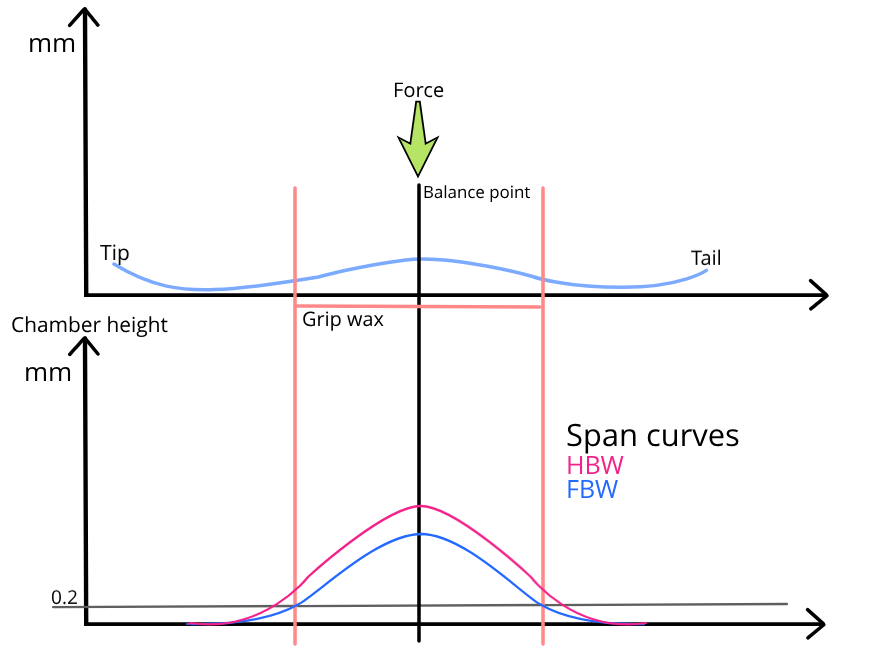
\includegraphics[width=1\textwidth]{figures/spancurve.png}
    \caption{An illustration of the span curves with HBW and FBW.}
    \label{fig:spancurve}
\end{figure}

\subsection{Camber height}
\label{subsec:camberheight}
The mechanical property camber height is described as the height from a flat surface to the sole of the ski, at a given load on the binding point(BP).
The purpose of looking at the camber height at FBW and HBW is to make sure that the contact area for gripping wax is being used to its full potential when a skier is kicking. And that the gripping wax does not get in contact with snow when the skier is gliding. Typically, the skis are marked on the side of the ski when the camber height is $0.2mm$ at both sides of the binding. Preferably, this height is when FBW is loaded. The purpose of the marks is to define the gripping area on the sole. Contact is defined as the camber height at $0.05mm$, this is when the gripping wax reaches the surface during kick-phase  \citep{breitschadel_variation_2012}. Furthermore, the change of camber height (in mm), at the BP when loaded from 0.5 to 1 times the BW was defined as the camber response \citep{breitschadel_technical_2014}. This was used to calculate the stiffness of the ski.

\subsection{Stiffness}
\label{subsec:stiffness}
The stiffness of the ski is related to the FBW and HBW when a pair of skis are chosen. The purpose of this mechanical property is to estimate the stiffness when the body weights are loaded. Stiffness contributes to giving the wanted camber heights for individual users with respect to their body weight and is important when finding a pair of matching skis for the different weather conditions. The stiffness, $k$, is the relation between the skiers half body weight and the camber response of the ski $(\frac{N}{mm})$ \citep{breitschadel_technical_2014}.

\subsection{Pressure Distribution}
\label{subsec:pressuredistribution}
The pressure distribution is a mechanical property that can be obtained by placing sensors along the ski as explained in Section \ref{sec:reasearchcontext}. The forces registered by the sensors represents the pressure from the ski on the surface at the point of the sensor placement. The purpose of measuring the forces at prefixed points where the sensors are placed is to find the weight loaded and how the weight distributes along the ski. This is also related to how much friction there is at the sensor location. Further on, pressure distribution property is of interest, because of the fluctuation the material is represented under stress, giving an indication of the ski quality. The pressure distribution can work as an additional property for finding the proper match of skis for an athlete. Nilsson et al. (2013) did research on how the force distribution changed when the loading point (center of mass) moved backwards from the original BP position. This investigation can also confirm the interest of looking at the ski characteristics when a skier goes over to a gliding-phase.

\begin{figure}
    \centering
    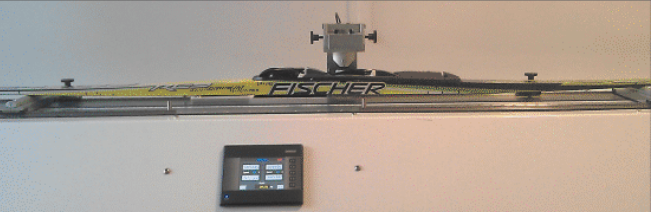
\includegraphics[width=1\textwidth]{figures/testbench.png}
    \caption{Ski test bench developed by Felix Breitschädel. Figure from \citep{breitschadel_technical_2014}}
    \label{fig:tbfelix}
\end{figure}

\section{Measurement devices}
\label{sec:measurementdevices}
The span curve is an important descriptor of the mechanical properties of the ski. Several measurement devices have been developed to efficiently and accurately measure the span curve and pressure distribution.

\subsection{Eiker måler}
\label{subsec:eiker}
The Eiker ski measurement device was originally developed for the winter Olympics in Lillehammer in 1994 by a Norwegian company called Ski-Test. The idea behind the Eiker-måler was to pair skis with similar flex, also referred to as span curve, and to find a reasonable match to the skier with regard to stiffness to weight ratio. Since the start of Ski-test, they have been developing their system with great success. Expanding the use to several countries, such as Sweden, Estland, Canada and the USA  to mention a few \citep{eiker_2018}. As instructed by the company, the electrical measurement device loads the ski with a skiers weight to HBW and FBW to mark the gliding zones and kicking zones for application of gliding wax and gripping wax respectively. An illustration of the device is shown in Figure \ref{fig:eikermåler}.

\begin{figure}
    \centering
    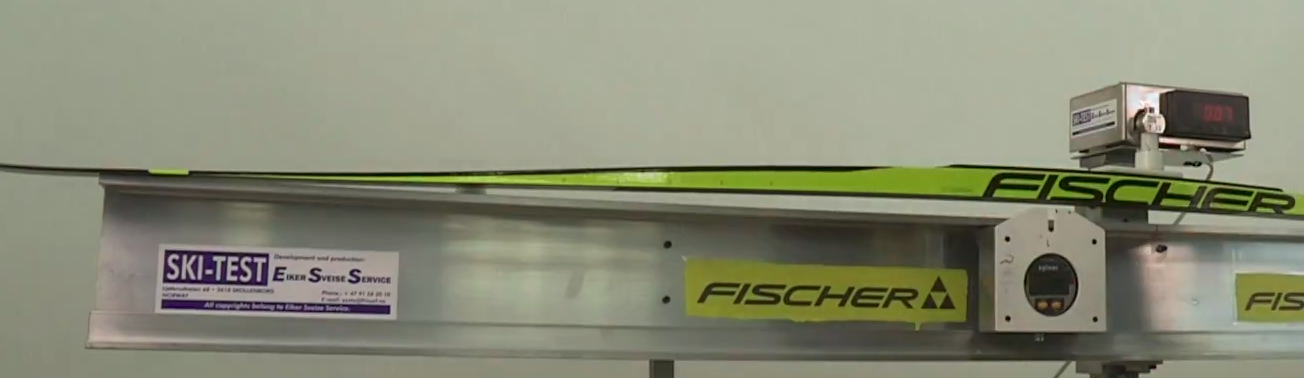
\includegraphics[width=0.9\textwidth]{figures/eiker.png}
    \caption{An illustration of the "Eiker-måler". Figure from \url{http://www.ski-test.no/instructions/}}
    \label{fig:eikermåler}
\end{figure}

\subsection{SkiSelector}
\label{subsec:skiselector}
The first SkiSelector system was developed for the winter Olympics in Turin in 2006. SkiSelector is a Swedish company, and have increased in popularity since 2006. During 2011, the SkiSelector Academy was founded for further development of the system. The system delivers a good overview of a skis mechanical properties such as grip, stiffness, camber characteristics and sliding properties. The goal of this system is to give the skier detailed information about the pair of skis on how the skis should be waxed for better grip and glide \citep{skiselector_2018}. The system can look very similar to the "Eiker-måler", but SkiSelector uses a computer and software to create a profile of each ski measured.

\subsection{IDT Sport - SkiAnalyzer}
\label{subsec:idt}
The SkiAnalyzer from IDT Sport delivers a complete measurement system with different software versions matching the user's experience. The measurements are based on laser technology to measure the camber height and stiffness. Through the software, the system outputs span and stiffness curves. Furthermore, at the end of a measurement, the user can save the measurement data to a database for later use \citep{idt_2018}. Thus, the information given by IDT Sport on the SkiAnalyzer is limited, the system seems to operate with the same precision as SkiSelector and Eiker Måler. The SkiAnalyzer is visualized in Figure \ref{fig:skianalyzer}.

\begin{figure}
    \centering
    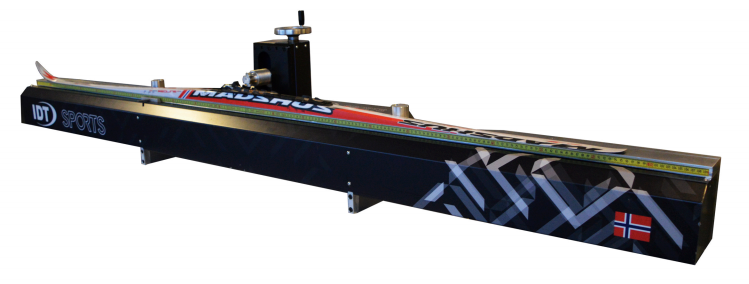
\includegraphics[width=0.9\textwidth]{figures/skianalyzer.png}
    \caption{An illustration of the SkiAnalyzer from IDT Sport. Figure from \url{https://www.idt.no/sport/produkter/skianalyzer/skianalyzer}}
    \label{fig:skianalyzer}
\end{figure}

\subsection{Gear West Signature Flex Tester}
\label{subsec:gwsft}
Gear West developed a system called Ski DNA \citep{skidna_2018}. Their system consists of three phases for choosing and measuring a cross-country ski, where the first phase is using hands and eyes when squeezing the skis. This is followed by the second phase where the skier will apply body weight in different positions on the ski. This is to find the ski pocket to ensure that the skis match each other. The third and last phase is to put the skis through the Flex Tester measurement bench. The measurement bench is designed to use loading cells to collect pressure distribution data. This data allows the system to check the quality of the flex, weight range and ideal snow condition for the skis.

\section{Chapter discussion}
In 2008, Bäckström investigated mechanical properties, such as span curve and pressure distribution, and the importance of finding the pressure distribution was further confirmed by Erkillä (1986). These mechanical properties are factors that are affecting the friction, $\mu$, between the skis and snow. Ekström (1980) showed that the friction, $\mu$, decreases with an increased camber value.


\section{Chapter conclusions}
\label{sec:backgroundconclusion}
Based on how the athlete's body weight is loaded on the ski, by for example different pronation of the foot. The thought is that a stiffer structure on the inside of the ski can be countered by an overpronation, resulting in an overall flatter running surface of a ski. With this in mind, it is possible that the friction is more evenly distributed on the surface, resulting in more evenly heat generation due friction and consistent water film due to frictional melting of snow.

On a last note, Breitschädel (2004) described in (\textbf{3.2.1 Methods for the ski analysis}) that a measurement uncertainty  with the Ski Analyzer \textit{Section \ref{subsec:idt}}, was effected by the ski running surface. Due to some skis running surface not being perfectly plane across the ski width because of twisting, some measurement areas on the ski could not register contact.

The Ski DNA system \textit{Section \ref{subsec:gwsft}}, is by far the most interesting system for this Master Thesis. More specifically the use of loading cells to measure the pressure distribution. The use of loading cells instead of laser technology to measure camber height is what makes Gear West Flex Tester's system unique.

This motivates the development of a measurement device to register both the pressure distribution and twisting in the ski structure. And, as mentioned, these twisting can also be considered a property of interest to match the force distribution from a specific skier weight transfer to the feet. As a student research project led by my supervisor Ole Marius Rindal and Jacob Norenberg, led to an idea to develop a measurement system using pressure sensitive films and a microcontroller to investigate pressure distribution in cross-country skis. This was shortly after canceled and resurrected as a master thesis at the University of Oslo, Department of Informatics.
A measurement device of this kind, is further explained and investigated in the following section.